\chapter{DCARC Control of the Actuator}
%===
Adaptive robust control (ARC) combines the asymptotic performance from parameter adaptation of adaptive control (MRAC)
with the transient performance of the nonlinear robust control techniques such as sliding mode
control(\cite{yao1997adaptive}, \cite{yao2010advanced}). This is primarily achieved by decoupling the stability of the
system from the adaptation law using projection to limit the domain of adaptation. Then a robust control law is
independently designed to ensure the transient performance across the entire domain of parameter values.

The projection operator also gives an added advantage of using non-gradient type adaptation laws like recursive least
squares (RLS) resulting in a faster parameter convergence (\cite{yao2003integrated}). Similarly, we can reduce the
effect of sensor noise on the adaptation and model compensation by designing the regression vectors for the parameter
estimation and model compensation solely based on the reference instead of the state measurements
(\cite{yao1998desired}, \cite{lu2008desired},\cite{hong2007globally}). This is particularly useful in the present
scenario where the RPM measurements are prone to significant noise. The stability is ensured by having additional
conditions on the stabilizing feedback. Such a design can also be used in the presence of actuator saturation.

The current study adopts the design and method of proof proposed in \cite{yao1998desired} for a first order nonlinear
system with friction and disturbance. The input saturation is implicitly considered in the reference system design,
filtering out the high-frequency components of the reference signal that can cause the actuator saturation due to model
compensation input. Additionally, the effects of saturation due to robust and stabilizing feedback can be explicitly
considered as in \cite{hong2007globally}.


\section{Control form and parameter bounds for the model}
From the experiments the system starts only at $u_\omega = 12.93$ which
is the minimum input required to overcome the static friction. This can be
verified as:
\begin{align}
     \lr{V_{in}^2  C_D u_\omega^2 }_{\lr{u_\omega = 12.93, V_{in} = 15.54}} = 1.4570 =  M_f \lr{\frac{V_{in}}{\hat V_{in}}}
\end{align}

Thus, expanding the range of $u_w$ from $[12.93, 67.23]$ to $[0, 67.23]$, the
dynamic model will now include the actual friction instead
of $M_f \lr{1 - \frac{V_{in}}{\hat V_{in}}}$. Rewriting equation~(\ref{eqn::nl_model}):

\begin{align}
    &J \dot \omega + b_m \omega + C_D \omega^2 + M_f = V_{in} \lr{b_m u_\omega + \hat V_{in} C_D u_\omega^2}
    \label{eqn::0_mdl}
\end{align}

Defining input to the system (u) as:
\begin{align}
    u &= \underbrace{\frac{1}{\hat J}\lr{\hat b_m u_\omega + \hat V_{in} \hat C_D u_\omega ^2}}_{g_u(u_\omega)} = \frac{K_r}{J} u_m  \label{eqn::ctrl_u}
\end{align}
Where $\hat \bullet$ are the estimated values of the parameters at the time of
calibration. Note that $\hat J$ is included in order to get the input into
appropriate scale.

Thus, $u$ is the actual PWM input to the inverter scaled by the ratio of the
torque constant and the winding resistance of the motor $\lr{\because K_r =
\frac{K_T}{R}}$.

Introducing the input definition (\ref{eqn::ctrl_u}) in to the nonlinear model
of the system (\ref{eqn::dyn_mdl}):
\begin{align*}
    \implies \dot \omega  &= -\frac{b_m}{J} \omega - \frac{C_D}{J} \omega^2 - \frac{M_f}{J} + V_{in} u
\end{align*}
Introducing the input and modelling uncertainties as $\Delta(u, \omega, t)$ (matched). Let,
$\bullet_{_J} = \frac{\bullet}{J}$. We have the control form of the model:
\begin{align}
   \dot \omega &= -b_{m_J} \omega - C_{D_J} \omega^2 - M_{f_J} + V_{in} u + \Delta(t, u, \omega) \label{eqn::ctrl_form}
\end{align}
The uncertainties in the input arise from the changes in the voltage from
calibration and the real system, the uncertainties in the parameter estimation
and higher-order input dynamics if any.

The control input calculated from the algorithm is not the actual hardware
input rather a nonlinear injective function of the hardware input. The
uniqueness in the mapping comes from the constraints in the range of input
values $(u > 0)$. From (\ref{eqn::ctrl_u}):
\begin{align*}
    &\hat V_{in} \hat C_D u_{\omega}^2 + \hat b_m u_\omega - \hat J u = 0\\
    %===
    \implies& u^{\pm}_\omega = \frac{-\hat b_m \pm \sqrt{\hat b_m ^2 + 4u \hat V_{in} \hat J \hat C_D}}{2 \hat V_{in} C_D}
    %===
\end{align*}
%===============================================================================
$\because \hat b_m, \hat C_D, \hat V_{in}, \hat J > 0 $ and $u_\omega > 0$ we have a unique mapping from $u$ to $u_w$:
\begin{align}
    u_\omega &= \underbrace{\frac{-\hat b_m + \sqrt{\hat b_m ^2 + 4u \hat V_{in} \hat J \hat C_D}}{2 \hat V_{in} \hat C_D}}_{g_u^+(u)}
    \label{eqn::u2uw}\\
    \implies u_p &= \frac{1}{a} \lr{g_u^+(u) - b} \qquad [\because u_\omega = a u_p + b \quad (\ref{eqn::uw_calib})]
\end{align}

Rewriting the (\ref{eqn::ctrl_form}) with the following definitions:
\begin{align*}
    &\Delta(t, x, u) = d_0 + d(t, x, u) \\
    %===
    & \theta_1 = C_{D_J}, \: \theta_2 = b_{m_J}, \: \theta_3 = M_{f_J} - d_0  \: \text{and,} \: b = V_{in}
    %===
\end{align*}
\begin{align}
    & \dot x = \underbrace{-\theta_1 x^2 -\theta_2 x - \theta_3}_{f(t, x)} + b u + d(t, x, u)
    \label{eqn::prm_ctrl_form}
\end{align}

Defining the following regression and parameter vectors:
\begin{align}
    \phi(x) &= \bm{ -x^2 & -x & -1}^T \\
    %===
    \theta &= \bm{\theta_1 & \theta_2 & \theta_3}^T = \bm{C_{D_J} & b_{m_J} & M_{f_J}-d_0}^T
    %===
\end{align}
The bounds on input
uncertainties are calculated based on the maximum and minimum values of the
parameter estimates at the calibration time (same as at realtime). From (\ref{eqn::ctrl_u}):
\begin{align*}
    \abs{\Delta}_{\max} &\leq \tilde \theta_{2M} \abs{u_\omega}_{\max} + \lr{\tilde b_M \abs{\theta_1}_{\max} + \abs{b}_{\max} \tilde \theta_{1M}}\abs{u_\omega}_{\max}^2  \\ &< 350 = d_M
\end{align*}

The Table~\ref{tab::parm_bounds} gives the minimum, maximum and nominal values
of the parameters of the equation (\ref{eqn::prm_ctrl_form}) from experimental
data:

\begin{table}[h]
    \caption{Summary of parameter bounds}
    \centering
    \begin{tabular}{r r r r}
        \hline \hline
        Parameter &Nominal & Minimum & Maximum \\ \hline
        $\theta_1$            &
        $0.0112$              &
        $0.0101$              &
        $0.0123$

        \\
        $\theta_2$               &
        $0$                      &
        $0$                      &
        $1$
        \\
        $\theta_3$                 &
        $407.44$                   &
        $0$                        &
        $750$
        \\
        $b$                        &
        $15.54$                    &
        $14.5$                     &
        $16.5$
        \\
        $d(t)$                   &
        $0$                      &
        $-700$                   &
        $700$
        \\
        \hline \hline
    \end{tabular}
    \label{tab::parm_bounds}
\end{table}

%=======================================================================================================================
\section{Actuation limits and the reference system design}
The actuator has hard limits beyond which the system doesn't function and
operational limits beyond which the system doesn't produce useful output. These are tabulated in Table~\ref{tab::actuator_limits}.
\begin{table}[h]
    \caption{Input and steady state output limits}
    \begin{center}
    \begin{tabular}{l r r r r}
        \hline \hline
        Limit & $u_p \,^*$ & $u_{\omega}$ & $u$ & $\omega$ \\ \hline
        Actual Lower         & 924  & 0     & 0        & 0\\
        Lower Start          & 1110 & 12.93 & 29.08    & 200.92 \\
        Operational Lower    & 1294 & 25.74 & 115.26   & 400 \\
        Operational Higher   & 1849 & 64.35 & 720.35   & 1000\\
        Actual Higher $(u_{\max})$& 1890 & 67.23 & 786.27   &  1044.56\\
        \hline \hline
    \end{tabular}
    \label{tab::actuator_limits}
    \end{center}
    $^*$PWM input in $\mu s$ at $400 \, Hz$ base frequency.
\end{table}
% ==============================================================================

The goal of feedback control design for the actuator is twofold:
(1) To compensate for input uncertainties, unmodeled disturbances, and model structure errors.
(2) To make the actuator track the response of a linear system (preferably a transfer function with no overshoot) within the operational limits. This ensures that the actuator achieves the maximum possible bandwidth in the presence of the mentioned uncertainties. Such a transfer function can be used as the actuator model for the drone control system design. Let the reference system be:
\begin{align*}
    G_{r}(s) &= \frac{\omega_{r}^2}{s^2 + 2s \zeta \omega_{r} + \omega_{r}^2}
    && \zeta = \frac{1}{\sqrt{2}} = 0.707
\end{align*}
The above reference system will also introduce a limit on the maximum rate of
change of angular velocity. By finding the peak magnitude of $s G_r(s)$, we have,
\begin{equation}
    \alpha(s) = s \omega(s) \;
    \implies \dot \omega_{\max} = \max \lr{\alpha(j \omega)}= \frac{1}{\sqrt{2}} \omega_r
\label{eqn::max_bandwidth}
\end{equation}
% ==============================================================================
% ==============================================================================
The input saturation imposes limitations on the maximum and minimum rate of
change of the angular velocity $(\omega)$. The primary goal of the reference
system design is to ensure that the input doesn't get saturated due to the
model compensation input $u_m$ (\ref{eqn::model_comp_input}). Let,
$u_{r}$ be the maximum available input for model compensation. This can be
calculated by maximum robust control input $(u_{s2})$ and the maximum
stabilizing feedback control input $(u_{s1})$.
\begin{align}
    u_{r} &= u_{\max} - \max {\lrf{u_{s1} + u_{s2}}}
\end{align}
$u_r$ can be calculated by finding the maximum value of $u_{s1}$ and $u_{s2}$
based on the equations (\ref{eqn::u_s1_def}, \ref{eqn::k_bound}) and
(\ref{eqn::robust_u}, \ref{eqn::h_bound}) respectively. The approximate upper
bound of $u_r$ is calculated to be $\leq 526.2$.

Thus, from the dynamic model (\ref{eqn::ctrl_form}), using the nominal parameter
values and removing the uncertainties and $u_r$, we have the
following bounds on the rate of change of the angular velocity within the
operational limits:
% ==============================================================================
\begin{enumerate}
    \item Maximum rate of increase:
        $\dot \omega^{+}_{max} = 10020.12 \; rad/s$
    \item Minimum rate of increase:
    $\dot \omega^{+}_{min} = 616.95 \; rad/s$
    \item Maximum rate of decrease:
        $\dot \omega^{-}_{max} = -11601.68 \; rad/s$
    \item Minimum rate of decrease:
        $\dot \omega^{-}_{min} = -2198.51 \; rad/s$
\end{enumerate}
% ==============================================================================
In order for the motor-propeller system to accurately track the response of a linear second-order system within the given input constraints, the maximum rate of change of the reference system state should be lower than the minimum rate of change in the actual system. This ensures that the system can keep up with the desired changes in the reference signal.
\begin{align}
    \abs{\dot \omega_{max}} &< \abs{\dot \omega^{+}_{min}} \quad
    \implies \omega_r <  872.5 \; rad/s
    \label{eqn::omega_r_lim}
\end{align}
% ==============================================================================
% ==============================================================================
The sampling due to the implementation of feedback would introduce its own
limitations on the maximum bandwidth of the reference system, namely, the
Nyquist frequency $(n_f = 125\,Hz)$ of sampling. The approximate inequality would be:
\begin{align}
    \omega_r < 2 \pi n_f = 785.4 \; rad/s
    \label{eqn::wr_lim_nf}
\end{align}
The above inequality (\ref{eqn::wr_lim_nf}), can be
flipped and combined with (\ref{eqn::omega_r_lim}) for using it as a design
limitation for the sampling system. Thus, the minimum sampling the requirement
for obtaining the maximum performance from the system as $2 \pi n_f > {\abs{\dot \omega^{\pm}_{min}}}$.
% ==============================================================================
% ==============================================================================

From the above inequalities on $\omega_r$, (\ref{eqn::wr_lim_nf}),
(\ref{eqn::omega_r_lim}), a conservative choice or $\omega_r$ as $200 \, rad/s$ is
chosen with $\zeta = {1}/{\sqrt{2}}$. The reason for choosing a lower value
is to have enough margins in inputs for the actual system to track the reference
system. Further gain optimizations through design iterations would lead to a
value close to its limits.

The reference system is discretized using the 'c2d' function in MATLAB using
zero-order-hold approach with a sampling frequency of $250 \; Hz$.

%=======================================================================================================================
\section{DCARC Design}
\subsection{Desired model compensation input}
The role of model compensation is to generate the required input for the
nominal plant state $(x)$ to track the desired trajectory $(x_d)$.
Let,
\begin{align}
    z &= x - x_d\\
    \implies \dot z &= \dot x - \dot x_d = \phi^T \theta +  bu + d - \dot x_d
    \label{eqn::error_dyn}
\end{align}

Considering only the nominal dynamics, i.e., assuming zero uncertainties ($d = 0$), the error dynamics can be simplified as follows:
\begin{align}
    \dot z &= \phi^T \theta + bu - \dot x_d
    \label{eqn::nom_error_dyn}
\end{align}
The total control input $u$ can be decomposed into $u_m$ (model compensation input) and $u_s$ (robust control input).
\begin{align}
    u &= u_m + u_s
\end{align}
The model compensation input in the present case is derived solely from the
reference trajectory dynamics and the model parameters. We have,
\begin{align}
    u_m &= \frac{1}{\hat b} \lr{\dot x_d - \phi^T(x_d) \hat \theta}
         = \frac{1}{\hat b} \lr{\dot x_d - \phi^T_d \hat \theta}
         \quad \lrb{\phi_d  = \phi(x_d)}
    \label{eqn::model_comp_input}
\end{align}
Substituting the above expression for $u_m$ in the nominal error dynamics
(\ref{eqn::nom_error_dyn}), let $\tilde b = \hat b - b$, we get:
\begin{align}
    \dot z
    &= \phi^T \theta - \phi^T_d \theta + \phi^T_d \theta - \phi^T_d \hat \theta + bu_s - \tilde b u_m
\end{align}
Let, $\tilde \phi = \phi(x) - \phi(x_d)$ and $\tilde \theta = \hat \theta -
\theta$. The error dynamics can be rewritten as:
\begin{align}
    \dot z &= \tilde \phi^T \theta - \phi^T_d \tilde \theta + bu_s - \tilde b u_m \label{eqn::error_dyn_model_comp}
\end{align}
It can be noted that as $\theta$ is unknown with known bounds, there exists a
known function $\delta_\phi(x, t)$ such that:
\begin{align}
    \abs{\tilde \phi^T \theta} &\leq \delta_\phi(x, t) \abs{z}
    \label{eqn::tl_phi_bound}
\end{align}


Further, let: $\phi_{du}^T = \bm{\phi_d^T & u_m}$ and $\theta_{b} = \bm{\theta^T
& b} \implies \tilde \theta_b = \bm{\tilde \theta^T & \tilde b}$
Substituting the above definitions in (\ref{eqn::error_dyn_model_comp}), we get:
\begin{align}
    \dot z &= \tilde \phi^T \theta - \phi_{du}^T \tilde \theta_b + bu_s
    \label{eqn::error_dyn_model_comp_2}
\end{align}
The robust feedback control input $u_s$ is further decomposed into two parts:
\begin{align}
    u_s &= u_{s1} + u_{s2}\\
    u_{s1} &= - k z \label{eqn::u_s1_def}
\end{align}
Substituting above expression for $u_s$ in the error dynamics
(\ref{eqn::error_dyn_model_comp_2}), we get:
\begin{align}
    \dot z + bk z &= \tilde \phi^T \theta - \phi_{du}^T \tilde \theta_b + bu_{s2}
    \label{eqn::error_feedback_dyn}
\end{align}
The robust feedback control input $u_{s2}$ is designed to account for the model
structure and input uncertainties (d) which are assumed to be zero in this
design. Thus analyzing the error dynamics (\ref{eqn::error_feedback_dyn}) with
$u_{s2} = 0$:
\begin{align*}
    \dot z + bk z &= \tilde \phi^T \theta - \phi_{du}^T \tilde \theta_b
\end{align*}
If $\tilde \theta_b$ asymptotically becomes zero, then the feedback gain of the
error dynamics should be large enough to compensate for $\tilde \phi^T \theta$.
From (\ref{eqn::tl_phi_bound}), we get the following condition for the zero
tracking error when the parametric uncertainties are zero:
\begin{align}
    bkz &\geq \delta_\phi(x, t) \abs{z}\\
    C1: \qquad \implies k &\geq \frac{1}{b}\delta_\phi(x, t) > \frac{1}{\hat b_{min}} \delta_\phi(x, t)
    \label{eqn::k_bound}
\end{align}

\subsection{Discontinuous projection based adaptation law}
The parameter estimation error $\tilde \theta_b$ can be reduced to zero asymptotically by using a gradient-based parameter adaptation law. This adaptation law is defined as follows:
\begin{align}
    \dot{\hat{\theta_b}} &= Proj_{\hat{\theta_b}}\lr{\Gamma \phi_{du}(t) z}
\end{align}
Where $\Gamma$ is a positive definite, diagonal adaption rate matrix.
We define, \itbf{Discontinuous projection mapping} $Proj()$ for a vector as follows:
\begin{align}
    &Proj_{\hat{\theta}} (\bullet) = \bm{Proj_{\hat \theta_1}(\bullet_1), &
                                        \hdots, &
                                        Proj_{\hat \theta_n}(\bullet_n)}
\end{align}
\begin{align}
    &Proj_{\hat \theta_i}(\bullet_i)
    = \begin{cases}
        0 & \text{if } \begin{cases}
                        \hat \theta_i &= \hat \theta_{i_{min}} \text{  and  } \bullet_i < 0\\
                        \hat \theta_i &= \hat \theta_{i_{max}} \text{  and  } \bullet_i > 0\\
                       \end{cases}\\
        \bullet_i & \text{otherwise}
    \end{cases}
\end{align}
The above mapping has the following properties:
    \begin{align}
        P1: & \: \hat{\pmb \theta} \in \bar \Omega_{\theta}=\{\hat{\pmb \theta} :
        \theta_{i_{min}} \leq \hat \theta_i \leq \theta_{i_{max}} \; \forall
        i\} \; \forall t\\
        %===
        P2: & \: \tilde{\pmb{\theta}} \left[ \Gamma^{-1} Proj_{\hat{\pmb\theta}}
        \lr{\Gamma \pmb \phi z} - \phi z \right] \leq 0 \: \forall t \quad
        [\tilde{\pmb{\theta}} = \hat{\pmb\theta} - \pmb \theta]
    \end{align}

The above adaptation law asymptotically reduces the errors due to parameter
estimation to zero. This can be proved by adding the following positive
definite term to the Lyapunov function, $\tilde \theta_b^T \Gamma^{-1} \tilde
\theta_b$, as shown in \cite{yao1998desired}.
%===============================================================================
%===============================================================================

%\subsection{Proof of stability and tracking performance when $d = 0$ \label{apx::dzero_stability}}

When $d = 0$ consider the following Lyapunov function:
\begin{align*}
    V &= \frac{1}{2} z^2 + \frac{1}{2} \tilde{\theta}_b^T \Gamma^{-1} \tilde{\theta}_b\\
    %===
    \implies \dot V &= z \dot z + \tilde \theta_b^T \Gamma^{-1} \dot{\hat \theta}_b\\
    %===
    &= z \lr{- bk z +  \tilde \phi^T \theta - \phi_{du}^T \tilde \theta_b}+ \tilde \theta_b^T \Gamma^{-1} \dot{\hat \theta}_b\\
    %===
    &\leq -bkz^2 + \delta_\phi z^2 - \tilde \theta_b^T \phi_{du} z + \tilde \theta_b^T \Gamma^{-1} \lr{\Gamma \phi_{du} z}\\
    %===
    &\leq z^2 \lr{-bk + \delta_\phi} < 0 \qquad \lrb{\because (\ref{eqn::k_bound})}\\
    \implies \dot V &< 0
\end{align*}
Thus,
\begin{itemize}
    \item $\dot V$ is negative semi-definite.
    \item $V$ has a lower bound $ \lrb{\because \geq 0}$.
\item $\dot V$ is uniform continuous $\lrb{\because \ddot V \leq \lr{-bk +
\delta_\phi}z \dot z }$.
    \item $\therefore$ For a bounded $x_d$, $z \in L_\infty$, $\tilde{
    \theta}_b \in L_{\infty}$ and $\dot z \in L_\infty$, $\ddot V \in L_\infty$.
\end{itemize}

Hence, the parameter estimates and tracking errors are bounded, and the system
is stable.

Also, since $V$ is non-decreasing and positive definite,
\begin{align*}
    &V(0) - V(t) \leq V(0) \:
    \implies -\int_0^t V d \tau \leq V(0)\\
    &\implies \int_0^t \lr{-bk + \delta_\phi} z^2 d \tau \leq V(0)\\
    &\implies \sqrt{\int_0^t \norm{z}^2 d \tau } \leq \sqrt{\frac{2 V(0)}{\lr{-bk + \delta_\phi}}} \leq \infty\\
    \therefore z &\in L_2
\end{align*}
From Barbalat's lemma, we have,
\begin{align*}
    \dot V \rightarrow 0 \quad z \rightarrow 0 \quad \text{as} \quad t \rightarrow 0
\end{align*}
Thus the parameter estimates are bounded, and the tracking error asymptotically
goes to zero as  $t \rightarrow 0$.


\subsection{Proof of stability and tracking performance when $d = 0$ \label{apx::dzero_stability}}

When $d = 0$ consider the following Lyapunov function:
\begin{align*}
    V &= \frac{1}{2} z^2 + \frac{1}{2} \tilde{\theta}_b^T \Gamma^{-1} \tilde{\theta}_b\\
    %===
    \implies \dot V &= z \dot z + \tilde \theta_b^T \Gamma^{-1} \dot{\hat \theta}_b\\
    %===
    &= z \lr{- bk z +  \tilde \phi^T \theta - \phi_{du}^T \tilde \theta_b}+ \tilde \theta_b^T \Gamma^{-1} \dot{\hat \theta}_b\\
    %===
    &\leq -bkz^2 + \delta_\phi z^2 - \tilde \theta_b^T \phi_{du} z + \tilde \theta_b^T \Gamma^{-1} \lr{\Gamma \phi_{du} z}\\
    %===
    &\leq z^2 \lr{-bk + \delta_\phi} < 0 \qquad \lrb{\because (\ref{eqn::k_bound})}\\
    \implies \dot V &< 0
\end{align*}
Thus,
\begin{itemize}
    \item $\dot V$ is negative semi-definite.
    \item $V$ has a lower bound $ \lrb{\because \geq 0}$.
\item $\dot V$ is uniform continuous $\lrb{\because \ddot V \leq \lr{-bk +
\delta_\phi}z \dot z }$.
    \item $\therefore$ For a bounded $x_d$, $z \in L_\infty$, $\tilde{
    \theta}_b \in L_{\infty}$ and $\dot z \in L_\infty$, $\ddot V \in L_\infty$.
\end{itemize}

Hence, the parameter estimates and tracking errors are bounded, and the system
is stable.

Also, since $V$ is non-decreasing and positive definite,
\begin{align*}
    &V(0) - V(t) \leq V(0) \:
    \implies -\int_0^t V d \tau \leq V(0)\\
    &\implies \int_0^t \lr{-bk + \delta_\phi} z^2 d \tau \leq V(0)\\
    &\implies \sqrt{\int_0^t \norm{z}^2 d \tau } \leq \sqrt{\frac{2 V(0)}{\lr{-bk + \delta_\phi}}} \leq \infty\\
    \therefore z &\in L_2
\end{align*}
From Barbalat's lemma, we have,
\begin{align*}
    \dot V \rightarrow 0 \quad z \rightarrow 0 \quad \text{as} \quad t \rightarrow 0
\end{align*}
Thus the parameter estimates are bounded, and the tracking error asymptotically
goes to zero as  $t \rightarrow 0$.

\subsection{Robust feedback control design}


Adding model uncertainties to the error dynamics (\ref{eqn::error_feedback_dyn}):
\begin{align}
    \dot z + bk z &=  \tilde \phi^T \theta + bu_{s2} - \lrb{ \phi_{du}^T \tilde \theta_b - d}
    \label{eqn::error_feedback_dyn_uncertain}
\end{align}

The left side of (\ref{eqn::error_feedback_dyn_uncertain}) represents the
stable nominal closed-loop dynamics. The terms in the brackets of the right-hand side represents the effect of all model uncertainties. Though these terms
are unknown, but they are bounded above with some known function h(x, t). The
goal of the robust feedback is to account for the uncertainties during the
transients and the steady state of parameter adaptation. Thus, $u_{s2}$ is
synthesized to satisfy the following two conditions:
\begin{align}
    C2:& \qquad z \lrb{-\phi_{du}^T \tilde \theta_b + d + b u_{s2}} \leq \varepsilon \\
    C3:& \qquad z b u_{s2} \leq 0
\end{align}
%===============================================================================
The function $h(x, t)$ is calculated as follows:
\begin{align}
    \abs{\phi_{du}^T \tilde \theta_b - d} &\leq h \implies h(x_d, t) = \abs{\phi_{du}^T(x_d, t)}  \tilde \theta_{bM} + 2 d_M
    \label{eqn::h_bound}
\end{align}
The robust feedback control input $u_{s2}$ is thus designed to satisfy the conditions $C2$ and $C3$ as follows:
\begin{align}
    u_{s_2} &= -\frac{1}{\hat b_{min}} S(h \sign(z)) \label{eqn::robust_u}\\
    %===
    S(h \sign(z)) &= h \sat \lr{ \frac{h}{4 \varepsilon} z} \quad [\text{Smoothing function}]\\
    %===
    \sat (x) &= \begin{cases}
        x  & \text{if  } \abs{x} \leq   1\\
        \sign(x) &  \text{otherwise}
    \end{cases}
\end{align}
The above defined smoothing function, $S(.)$, has the following properties:
\begin{align}
    P3: & \quad z S(h \sign(z)) = z h \sat \lr{\frac{h}{4 \varepsilon} z} \geq 0\\
    P4: & \quad z \left[h \sign(z) - S(h\sign(z)) \right] \text{  is bounded.}
\end{align}

The robust control input definition (\ref{eqn::robust_u}) satisfies the
conditions $C2$ and $C3$ as long as $P3, P4$ are valid (\cite{yao1998desired}).

\subsection{Proof of stability and tracking performance when $d \neq 0$}
Consider the following Lyapunov function:
\begin{align*}
    V &= \frac{1}{2} z^2\\
    \implies \dot V &= z \dot z = z \lr{-kbz + \tilde \phi^T \theta - \phi_{du}^T \tilde \theta_b + d + b u_{s2}}\\
    %===
    &= -(kb - \delta_{\phi})z^2 + z \lr{- \phi_{du}^T \tilde \theta_b + d + b u_{s2}}\\
    &\leq -(kb - \delta_{\phi}) z^2 + \varepsilon \qquad [\because C3] \\
    \implies \dot V &\leq -k_p z^2 + \varepsilon = - 2 k_p V + \varepsilon
\end{align*}
By applying comparison lemma, the upper bound can be found from the forced
response of the following ODE:
\begin{align*}
    &\dot V + 2 k_p V = \varepsilon\\
    &\implies sV - V(0) + 2 k_p V = \varepsilon\\
    &\implies V = \frac{V(0)}{s + 2 k_p} + \frac{\varepsilon}{2 k_p}\\
    &\implies V(t) = V(0)e^{2 k_p t} + \int_0^t{e^{2 k_p (t-\tau)} \varepsilon(\tau) d\tau}\\
    &\implies \frac{1}{2} z^2 = \frac{1}{2} z(0)^2 e^{2 k_p t} + \int_0^t{e^{2 k_p (t-\tau)} \varepsilon(\tau) d\tau}\\
    %===
    &\implies \abs{z(t)}^2 = z(0)^2 e^{2 k_p t} +2 \int_0^t{e^{2 k_p (t-\tau)} \varepsilon(\tau) d\tau}\\
    &\qquad \qquad \leq z(0)^2 e^{2 k_p t} + \frac{\varepsilon_M}{k_p} \left[1 -  e^{2 k_p t} \right]
    %==
\end{align*}
This the system is stable, and the transient response is bounded that
exponentially converges to $\frac{\varepsilon}{k_p}$.

%\subsection{Controller parameter selection and tuning}

The controller parameters for the DCARC design are selected based on the
conditions C1-C3. The controller parameters are given in Table~\ref{tab::ctrl_prm}.
\begin{table}[H]
    \caption{Parameters for the DCARC design}
    \label{tab::ctrl_prm}
    \centering
    \begin{tabular}{c l}
        \hline \hline
        Parameter & Value \\
        \hline
        $k$ & $2.0$ \\
        $h$ & $1000$ \\
        $\varepsilon$ & $10$ \\
        $\Gamma$ & $diag\lr{\mat{1.1e-10, & 5e-05,& 3.75,& 2e-04}}$\\
        \hline\hline
    \end{tabular}
\end{table}

%=======================================================================================================================
\section{Experimental Results}
The controller's performance was evaluated by tracking a square wave reference signal with a half-period of 5 seconds. The system's response, as shown in Figure~\ref{fig::response}, aligns with the reference system design. The system was able to track the reference signal without significant transient tracking errors (Figure~\ref{fig::error_inputs}) due to input saturation. The steady-state error remained within the bounds of the RPM sensor's resolution (\cite{seshaIdent}).

The high-frequency oscillations in the tracking response are primarily
attributed to the RPM sensors resolution $(\approx 50 \, rad/s)$ and the
switching in robust control input to compensate for the resulting tracking
error. This can be further smoothed by increasing the value of $\varepsilon$,
although this may result in poorer transient performance. The estimated
parameters converged to the actual values (Figure~\ref{fig::param_est}). The
rate of convergence can be further t improved by tuning the adaptation rate
matrix with appropriate scaling based on the ranges of individual parameters.

\begin{figure}[H]
    \centering
    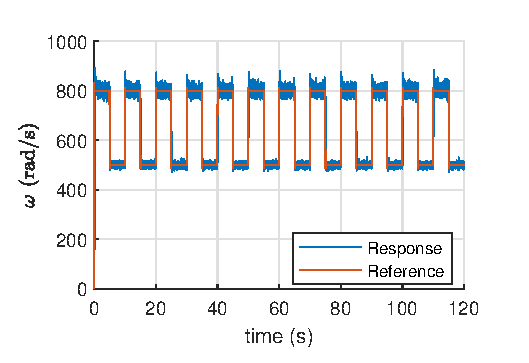
\includegraphics[width = 0.49\textwidth]{Part2/figs/4_figs/results/response.eps}
    \caption{Controller response to a square wave reference signal}
    \label{fig::response}
\end{figure}

\begin{figure}[H]
    \begin{minipage}{0.49\textwidth}
        \begin{figure}[H]
            \centering
            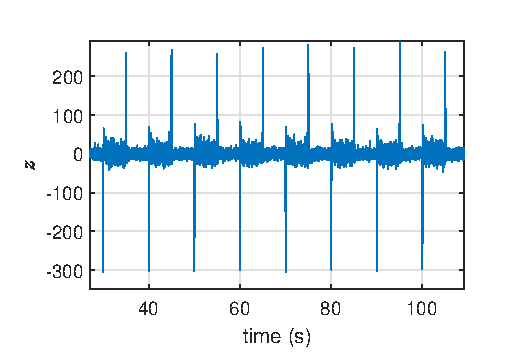
\includegraphics[width=\textwidth]{Part2/figs/4_figs/results/z.eps}
        \end{figure}
    \end{minipage}
    \begin{minipage}{0.49\textwidth}
        \begin{figure}[H]
            \centering
            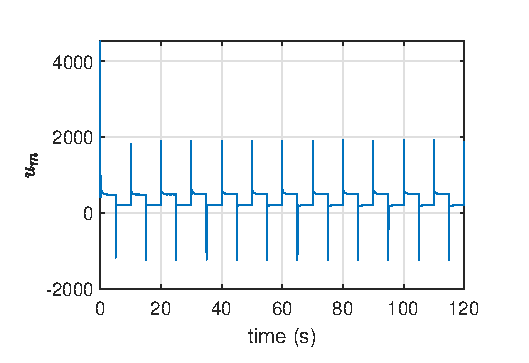
\includegraphics[width=\textwidth]{Part2/figs/4_figs/results/um.eps}
        \end{figure}
    \end{minipage}
\end{figure}
\begin{figure}[H]
    \begin{minipage}{0.49\textwidth}
        \begin{figure}[H]
            \centering
            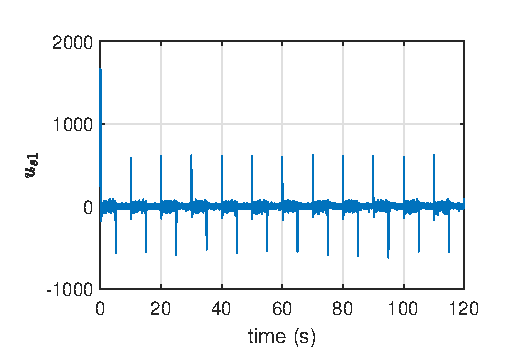
\includegraphics[width=\textwidth]{Part2/figs/4_figs/results/us1.eps}
        \end{figure}
    \end{minipage}
    \begin{minipage}{0.49\textwidth}
        \begin{figure}[H]
            \centering
            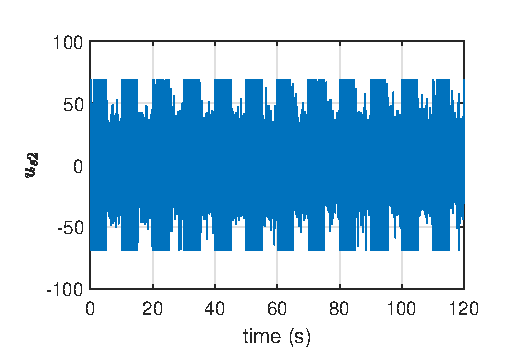
\includegraphics[width=\textwidth]{Part2/figs/4_figs/results/us2.eps}
        \end{figure}
    \end{minipage}
    \caption{Tracking error and control inputs}
    \label{fig::error_inputs}
\end{figure}


\begin{figure}[H]
    \begin{minipage}{0.49\textwidth}
        \begin{figure}[H]
            \centering
            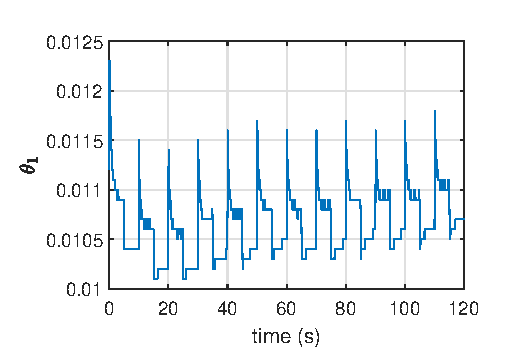
\includegraphics[width=\textwidth]{Part2/figs/4_figs/results/th1.eps}
        \end{figure}
    \end{minipage}
    \begin{minipage}{0.49\textwidth}
        \begin{figure}[H]
            \centering
            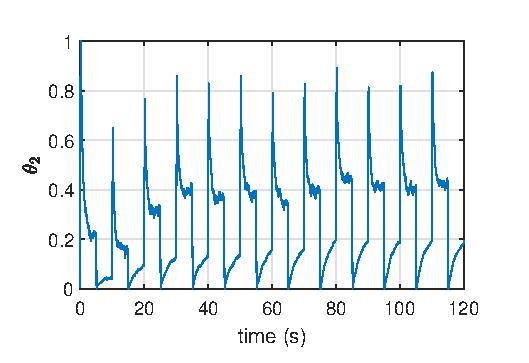
\includegraphics[width=\textwidth]{Part2/figs/4_figs/results/th2.eps}
        \end{figure}
    \end{minipage}
\end{figure}
\begin{figure}[H]
    \begin{minipage}{0.49\textwidth}
        \begin{figure}[H]
            \centering
            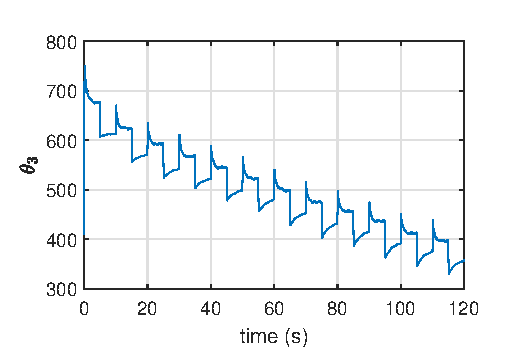
\includegraphics[width=\textwidth]{Part2/figs/4_figs/results/th3.eps}
        \end{figure}
    \end{minipage}
    \begin{minipage}{0.49\textwidth}
        \begin{figure}[H]
            \centering
            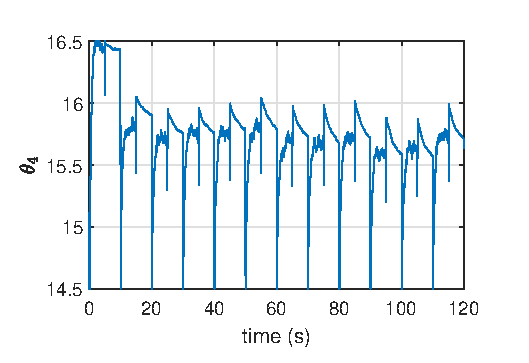
\includegraphics[width=\textwidth]{Part2/figs/4_figs/results/th4.eps}
        \end{figure}
    \end{minipage}
    \caption{Parameter estimation results}
    \label{fig::param_est}
\end{figure}

